\chapter{Introduction}

Within the large framework of complex systems, stochastic processes lend us a hand to decypher properties of living systems, bridging randomness with structured behaviour.
This processes are used to model the dynamics of systems which evolve randomly in time. This is why they are ideal for describing natural phenomena such as 
the spread of diseases \cite{Chowell}, social networks \cite{castellano2009statistical} or ecological systems \cite{azaele2016statistical}. Mathematically, a stochastic process
is a collection of random variables \cite{McKane}, generally ordered in time $ \{X_t\}_{t \in T} $, where $t$ is the time and $X_t$ is the system state at time $t$. $T$ is the time index set, 
which can be discrete or continuous, in this work we will focus on the discrete case because we are interested in the study of point (Hawkes) processes for modeling neurons. 

Point processes are a type of stochastic process that describe the occurrence of events in time or space. We will be interested in time point processes because 
we are going to model the spiking activity of neurons. For our purposes, they will be characterized by two parameters, the time of occurrence
of the events $t_k$ and the intensity or rate of occurrence of these events $\lambda$. This rate tell us how likely is that an event occurs at time $t$ given the history of the process 
(probability density function, PDF) as pictured in Figure \ref{f:point_process}.

\begin{figure}[H]
    \centering
    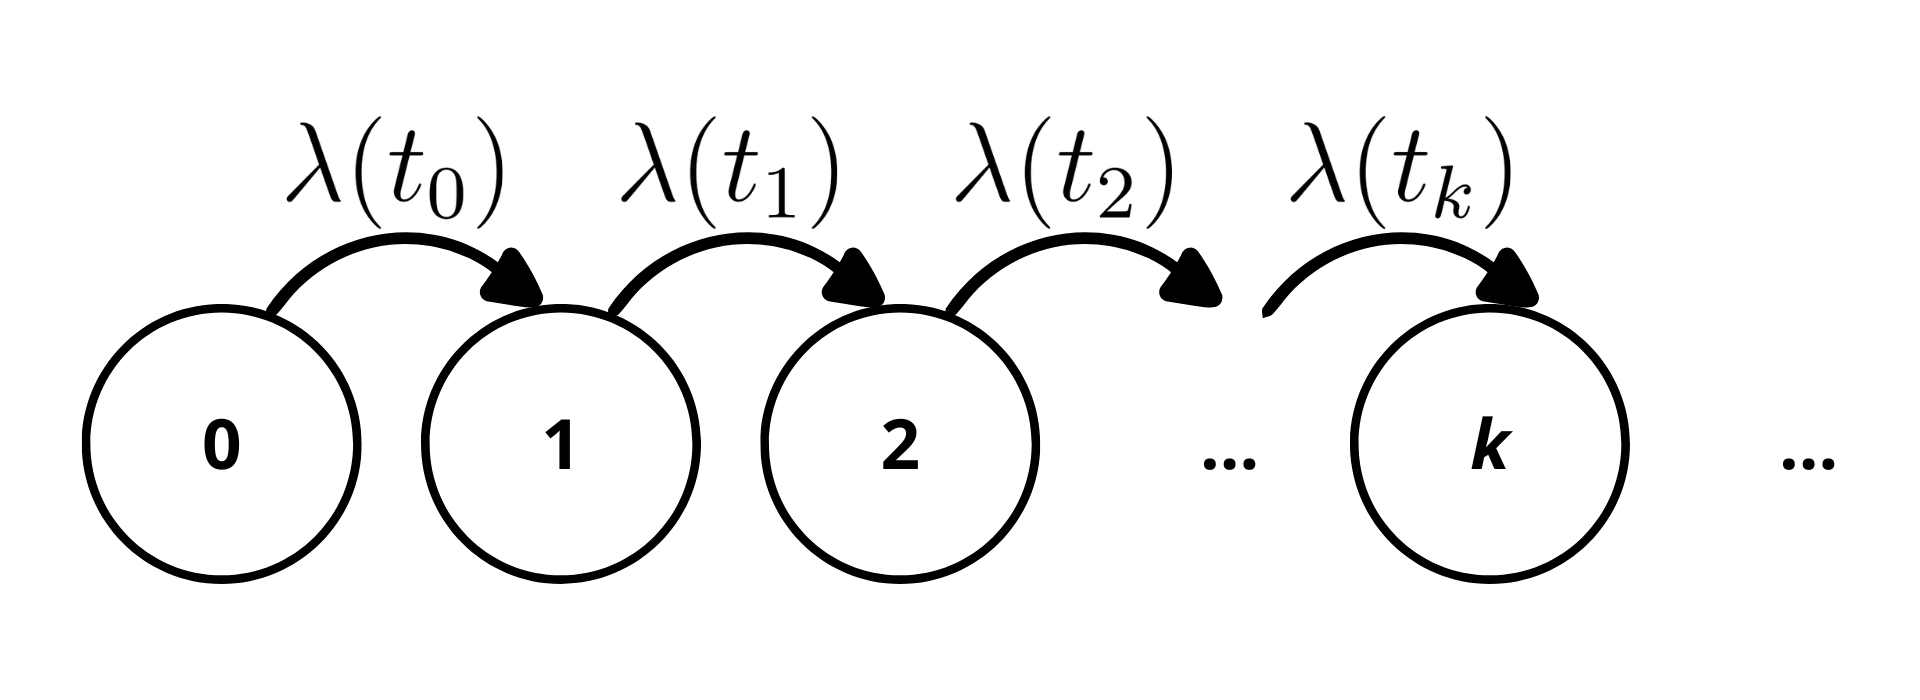
\includegraphics[width=0.7\textwidth]{Point process.png}
    \caption{Representation of a point process. The intensity function $\lambda(t)$ is a time-dependent function.}
    \label{f:point_process}
\end{figure}

In general, the rate is a function of the history of the process, which makes the process non-Markovian. But in our case, it will be a Markovian process, which means that the rate depends 
only on the last event that occurred as we will see. An example of a Markovian point process is the Poisson process, which is a simple and one of the most studied point processes because 
they are present in many everyday situations such as the arrival of customers at a store, occurrence of defects on a Production line. They are also present in physics, for instance, 
the decay of radioactive particles or the arrival of photons at a detector. These processes are characterized by a constant rate of occurrence of events making them memoryless and Markovian.
MIRAR INFO DE POISSON EN WIKIPEDIA

In most cases, the motivation of study of point processes is counting them, but in our case we also are interested in the time of occurrence of the events
which will let us define bursts or avalanches of activity that we will use to describe the dynamics of the system. 

PONER AQUÍ ALGUNA FIGURA GENERADA POR MI